\documentclass[mstat,12pt]{unswthesis}


\newlength{\cslhangindent}
\setlength{\cslhangindent}{1.5em}
\newenvironment{CSLReferences}%
  {}%
  {\par}

%%%%%%%%%%%%%%%%%%%%%%%%%%%%%%%%%%%%%%%%%%%%%%%%%%%%%%%%%%%%%%%%%%
% 
% OK...Now we get to some actual input.  The first part sets up
% the title etc that will appear on the front page
%
%%%%%%%%%%%%%%%%%%%%%%%%%%%%%%%%%%%%%%%%%%%%%%%%%%%%%%%%%%%%%%%%%

\title{Group Project Plan by Group G\\[0.5cm]A Data Science Approach to
Forecast Electricity Consumption in Australia}

\authornameonly{Kourosh Shaban (z5016011), Kin Ieng Cheang (z5003196), \\ Alexander Hodges (z5411346), Zining Wang (z5401010)}

\author{\Authornameonly}

\copyrightfalse
\figurespagefalse
\tablespagefalse

%%%%%%%%%%%%%%%%%%%%%%%%%%%%%%%%%%%%%%%%%%%%%%%%%%%%%%%%%%%%%%%%%
%
%  And now the document begins
%  The \beforepreface and \afterpreface commands puts the
%  contents page etc in
%
%%%%%%%%%%%%%%%%%%%%%%%%%%%%%%%%%%%%%%%%%%%%%%%%%%%%%%%%%%%%%%%%%%


%%%%%%%%%%%%%%%%%%%%%%%%%%%%%%%%%%%%%%%%%%%%%%%%%%%%%%%%%%%%%%%%%%%%%%%
%
%  A small sample UNSW Coursework Masters thesis file.
%  Any questions to Ian Doust i.doust@unsw.edu.au and/or Gery Geenens ggeenens@unsw.edu.au
%
%%%%%%%%%%%%%%%%%%%%%%%%%%%%%%%%%%%%%%%%%%%%%%%%%%%%%%%%%%%%%%%%%%%%%%%
%
%  The first part pulls in a UNSW Thesis class file.  This one is
%  slightly nonstandard and has been set up to do a couple of
%  things automatically
%
 
%%%%%%%%%%%%%%%%%
%% Precisely one of the next four lines should be uncommented.
%% Choose the one which matches your degree, uncomment it, and comment out the other two!
%\documentclass[mfin,12pt]{unswthesis}    %%  For Master of Financial Mathematics 
%\documentclass[mmath,12pt]{unswthesis}   %%  For Master of Mathematics
%\documentclass[mstat,12pt]{unswthesis}  %%  For Master of Statistics
%%%%%%%%%%%%%%%%%



\linespread{1}
\usepackage{amsfonts}
\usepackage{amssymb}
\usepackage{amsthm}
\usepackage{latexsym,amsmath}
\usepackage{graphicx}
\usepackage{afterpage}
\usepackage[colorlinks]{hyperref}
 \hypersetup{
     colorlinks=true,
     linkcolor=blue,
     filecolor=blue,
     citecolor= black,      
     urlcolor=cyan,
     }
\usepackage{textcomp}
\usepackage{longtable}
\usepackage{booktabs}

%%%%%%%%%%%%%%%%%%%%%%%%%%%%%%%%%%%%%%%%%%%%%%%%%%%%%%%%%%%%%%%%%
%
%  The following are some simple LaTeX macros to give some
%  commonly used letters in funny fonts. You may need more or less of
%  these
%
\newcommand{\R}{\mathbb{R}}
\newcommand{\Q}{\mathbb{Q}}
\newcommand{\C}{\mathbb{C}}
\newcommand{\N}{\mathbb{N}}
\newcommand{\F}{\mathbb{F}}
\newcommand{\PP}{\mathbb{P}}
\newcommand{\T}{\mathbb{T}}
\newcommand{\Z}{\mathbb{Z}}
\newcommand{\B}{\mathfrak{B}}
\newcommand{\BB}{\mathcal{B}}
\newcommand{\M}{\mathfrak{M}}
\newcommand{\X}{\mathfrak{X}}
\newcommand{\Y}{\mathfrak{Y}}
\newcommand{\CC}{\mathcal{C}}
\newcommand{\E}{\mathbb{E}}
\newcommand{\cP}{\mathcal{P}}
\newcommand{\cS}{\mathcal{S}}
\newcommand{\A}{\mathcal{A}}
\newcommand{\ZZ}{\mathcal{Z}}
%%%%%%%%%%%%%%%%%%%%%%%%%%%%%%%%%%%%%%%%%%%%%%%%%%%%%%%%%%%%%%%%%%%%%
%
% The following are much more esoteric commands that I have left in
% so that this file still processes. Use or delete as you see fit
%
\newcommand{\bv}[1]{\mbox{BV($#1$)}}
\newcommand{\comb}[2]{\left(\!\!\!\begin{array}{c}#1\\#2\end{array}\!\!\!\right)
}
\newcommand{\Lat}{{\rm Lat}}
\newcommand{\var}{\mathop{\rm var}}
\newcommand{\Pt}{{\mathcal P}}
\def\tr(#1){{\rm trace}(#1)}
\def\Exp(#1){{\mathbb E}(#1)}
\def\Exps(#1){{\mathbb E}\sparen(#1)}
\newcommand{\floor}[1]{\left\lfloor #1 \right\rfloor}
\newcommand{\ceil}[1]{\left\lceil #1 \right\rceil}
\newcommand{\hatt}[1]{\widehat #1}
\newcommand{\modeq}[3]{#1 \equiv #2 \,(\text{mod}\, #3)}
\newcommand{\rmod}{\,\mathrm{mod}\,}
\newcommand{\p}{\hphantom{+}}
\newcommand{\vect}[1]{\mbox{\boldmath $ #1 $}}
\newcommand{\reff}[2]{\ref{#1}.\ref{#2}}
\newcommand{\psum}[2]{\sum_{#1}^{#2}\!\!\!'\,\,}
\newcommand{\bin}[2]{\left( \begin{array}{@{}c@{}}
				#1 \\ #2
			\end{array}\right)	}
%
%  Macros - some of these are in plain TeX (gasp!)
%
\newcommand{\be}{($\beta$)}
\newcommand{\eqp}{\mathrel{{=}_p}}
\newcommand{\ltp}{\mathrel{{\prec}_p}}
\newcommand{\lep}{\mathrel{{\preceq}_p}}
\def\brack#1{\left \{ #1 \right \}}
\def\bul{$\bullet$\ }
\def\cl{{\rm cl}}
\let\del=\partial
\def\enditem{\par\smallskip\noindent}
\def\implies{\Rightarrow}
\def\inpr#1,#2{\t \hbox{\langle #1 , #2 \rangle} \t}
\def\ip<#1,#2>{\langle #1,#2 \rangle}
\def\lp{\ell^p}
\def\maxb#1{\max \brack{#1}}
\def\minb#1{\min \brack{#1}}
\def\mod#1{\left \vert #1 \right \vert}
\def\norm#1{\left \Vert #1 \right \Vert}
\def\paren(#1){\left( #1 \right)}
\def\qed{\hfill \hbox{$\Box$} \smallskip}
\def\sbrack#1{\Bigl \{ #1 \Bigr \} }
\def\ssbrack#1{ \{ #1 \} }
\def\smod#1{\Bigl \vert #1 \Bigr \vert}
\def\smmod#1{\bigl \vert #1 \bigr \vert}
\def\ssmod#1{\vert #1 \vert}
\def\sspmod#1{\vert\, #1 \, \vert}
\def\snorm#1{\Bigl \Vert #1 \Bigr \Vert}
\def\ssnorm#1{\Vert #1 \Vert}
\def\sparen(#1){\Bigl ( #1 \Bigr )}

\newcommand\blankpage{%
    \null
    \thispagestyle{empty}%
    \addtocounter{page}{-1}%
    \newpage}

%%%%%%%%%%%%%%%%%%%%%%%%%%%%%%%
%
% These environments allow you to get nice numbered headings
%  for your Theorems, Definitions etc.  
%
%  Environments
%
%%%%%%%%%%%%%%%%%%%%%%%%%%%%%%%

\newtheorem{theorem}{Theorem}[section]
\newtheorem{lemma}[theorem]{Lemma}
\newtheorem{proposition}[theorem]{Proposition}
\newtheorem{corollary}[theorem]{Corollary}
\newtheorem{conjecture}[theorem]{Conjecture}
\newtheorem{definition}[theorem]{Definition}
\newtheorem{example}[theorem]{Example}
\newtheorem{remark}[theorem]{Remark}
\newtheorem{question}[theorem]{Question}
\newtheorem{notation}[theorem]{Notation}
\numberwithin{equation}{section}

%%%%%%%%%%%%%%%%%%%%%%%%%%%%%%%%%%%%%%%%%%%%%%%%%%%%%%%%%%%%%%%%%%
%
%  If you've got some funny special words that LaTeX might not
% hyphenate properly, you can give it a helping hand:
%

\hyphenation{Mar-cin-kie-wicz Rade-macher}






\usepackage{multirow}
\usepackage[table,xcdraw]{xcolor}
\usepackage{array}
\usepackage{colortbl}
\usepackage{graphicx}
\pagestyle{empty}

\begin{document}

\beforepreface

\prefacesection{Abstract}

A first assessed activity will be the Group Project Plan (20\%). The
first step is to delimit the problem which will be studied. You should
understand and define your own overall problem and propose a solution.
Having only a short time to complete the project, it is crucial that the
problem that will be studied is well defined. The approach to solve the
problem should be original, so it will be necessary to carry out a
preliminary literature review. This will prevent any plagiarism. This
will also enable you to situate the project in a more global context. At
this stage, one can identify potential approaches and software that will
be used to solve the problem. It is necessary to plan any simulation
carefully and to decide what statistical analyses will have to be
carried out. All the sub-steps of the project should be planned
precisely (a detailed schedule will be created). A kind of short draft
version of your final report, consisting of a three-page proposal
(excluding the mandatory pages devoted to the title, abstract, contents
and references) will be submitted and discussed with one of the
instructors at the end of Week 1 or in a clear definition of the problem
you plan to study; a clear description of the data format and their
storage; a clear description of the relevant data (variables, missing
and corrupt values, etc.); the level of difficulty of the chosen data
sets (size, complexity, messiness) and its relevance for the chosen
problem; the appropriate choice of software and statistical methods to
solve your research questions; a clear description of the role of each
team member with a proper justification; the precision of your scheduled
activities.

%\afterpage{\blankpage}


\afterpreface





%%%%%%%%%%%%%%%%%%%%%%%%%%%%%%%%%%%%%%%%%%%%%%%%%%%%%%%%%%%%%%%%%%
%
% Now we can start on the first chapter
% Within chapters we have sections, subsections and so forth
%
%%%%%%%%%%%%%%%%%%%%%%%%%%%%%%%%%%%%%%%%%%%%%%%%%%%%%%%%%%%%%%%%%%



%%%%%%%%%%%%%%%%%%%%%%%%%%%%%%%%%%%%%

%\afterpage{\blankpage}


\setcounter{chapter}{1}
\renewcommand\thesection{\arabic{section}}

\hypertarget{introduction-and-motivation}{%
\section{Introduction and
Motivation}\label{introduction-and-motivation}}

You should describe the problem in your own words and motivate its
importance. Your description should be clear for a reader not familiar
with the problem (e.g., a student in your discipline but who is not
involved in the course, another professor from your school who is not
teaching this course). The idea is that you explain clearly what you
have understood about what exactly is the problem after having listened
to the project provider, and after potential discussions with the
sponsor and/or your lecturers. Each team can define its own specific
problem in the context of the global problem and associated data sets
provided by the ``client.''

\bigskip

Then, briefly describe how you intend to solve the problem (e.g.,
compare several existing methodologies, apply specific statistical
techniques, etc.).

\hypertarget{brief-literature-review}{%
\section{Brief Literature Review}\label{brief-literature-review}}

Survey the most related work you have found in the literature. Due to
space restrictions, describe only the most relevant work and discuss its
connections to your work. Describe the methods employed in the related
work, as well as the employed measure of success.

\bigskip

In order to incorporate your own references in this report, we strongly
advise you use BibTeX. Your references then need to be recorded in the
file \texttt{references.bib}, and cited as follows {[}1{]}.

\hypertarget{methods-software-and-data-description}{%
\section{Methods, Software and Data
Description}\label{methods-software-and-data-description}}

You should describe the techniques you intend to use and why you have
selected these techniques. Also, describe the software and libraries
that you will need to implement your analyses. You can revise this later
since this is an initial proposal. Finally, provide a clear description
of the relevant data (format, storage, variables, messiness, size,
complexity) and its relevance for the chosen problem.

%%%%%%%%%%%%%%%%%%%%%%%%JoshJosh%%%%%%%%%%%%%%%%%%%%%%%%%%%%%%%%%%%%%%%%%%%%%%%%%%%%%%%%%%%%%%%%%%%%%%%%%%%%%%%%%%%%%%%%%%%%%%%%%%%%%%%%%%%
%Preamble
%\documentclass[10pt,a4paper,oneside]{report}
%\usepackage{amsmath,amsthm,amssymb}
%\usepackage{multirow}
%\usepackage[table,xcdraw]{xcolor}
%\usepackage{array}
%\usepackage{colortbl}
%\usepackage{graphicx}
%\pagestyle{empty}

\hypertarget{activities-and-schedule}{%
\section{Activities and Schedule}\label{activities-and-schedule}}
\setlength{\parindent}{0pt} %

%\vspace{-4cm}\section{Activities and Schedule}

\textbf{Description of Activity Allocation:}
Our project has 13 main activities, five of which are done jointly by all team members and the other seven are allocated to the most suitable team members based on their strengths. For example, Kin is good at research and has flexible working hours, so she was selected as the leader of our team, responsible for making Literature Review, deciding research questions and presentation slides. The following table shows the strengths of the group members and the activities they are responsible for.
\begin{table}[htbp]
	\resizebox{1\textwidth}{!}{
	\begin{tabular}{|1|cll|}
		\hline
		\multicolumn{1}{|c|}{Tasks} & \multicolumn{1}{c|}{\cellcolor[HTML]{FFFFFF}Members Name} & \multicolumn{1}{c|}{Members Roles} & \multicolumn{1}{c|}{Members Strengths and Experiences} \\ \hline
		Decide roles of members & \multicolumn{3}{c|}{All Members} \\ \hline
		Decide research question & \multicolumn{3}{c|}{All Members} \\ \hline
		Write project plan & \multicolumn{3}{c|}{All Members} \\ \hline
		Write report & \multicolumn{3}{c|}{All Members} \\ \hline
		Source external data & \multicolumn{3}{c|}{All Members} \\ \hline
		Record presentation & \multicolumn{3}{c|}{All Members} \\ \hline
		& \multicolumn{1}{c|}{Kin Cheang} & \multicolumn{1}{c|}{Team Leader} & Coding, Research, Mathematics \\ \cline{2-4} 
		\multirow{-2}{*}{Literature review} & \multicolumn{1}{c|}{Zining Wang} & \multicolumn{1}{c|}{Data Analyst} & Coding, Data visualization, Research \\ \hline
		& \multicolumn{1}{c|}{Alexander Hodges} & \multicolumn{1}{c|}{} & Coding, Machine learning, Mathematics \\ \cline{2-2} \cline{4-4} 
		\multirow{-2}{*}{Research methods and software} & \multicolumn{1}{c|}{Zining Wang} & \multicolumn{1}{c|}{\multirow{-2}{*}{Data Analyst}} & Coding, Data visualization, Research \\ \hline
		& \multicolumn{1}{c|}{Kourosh Shaban} & \multicolumn{1}{c|}{} & Coding, Machine learning, Mathematics \\ \cline{2-2} \cline{4-4} 
		& \multicolumn{1}{c|}{Alexander Hodges} & \multicolumn{1}{c|}{} & Coding, Machine learning, Mathematics \\ \cline{2-2} \cline{4-4} 
		\multirow{-3}{*}{Data preparation} & \multicolumn{1}{c|}{Zining Wang} & \multicolumn{1}{c|}{\multirow{-3}{*}{Data Analyst}} & Coding, Data visualization, Research \\ \hline
		& \multicolumn{1}{l|}{Kourosh Shaban} & \multicolumn{1}{l|}{} & Coding, Machine learning, Mathematics \\ \cline{2-2} \cline{4-4} 
		& \multicolumn{1}{l|}{Alexander Hodges} & \multicolumn{1}{l|}{} & Coding, Machine learning, Mathematics \\ \cline{2-2} \cline{4-4} 
		\multirow{-3}{*}{Data analysis} & \multicolumn{1}{l|}{Zining Wang} & \multicolumn{1}{l|}{\multirow{-3}{*}{Data Analyst}} & Coding, Data visualization, Research \\ \hline
		& \multicolumn{1}{l|}{Kourosh Shaban} & \multicolumn{1}{l|}{} & Coding, Machine learning, Mathematics \\ \cline{2-2} \cline{4-4} 
		& \multicolumn{1}{l|}{Alexander Hodges} & \multicolumn{1}{l|}{} & Coding, Machine learning, Mathematics \\ \cline{2-2} \cline{4-4} 
		\multirow{-3}{*}{Modelling} & \multicolumn{1}{l|}{Zining Wang} & \multicolumn{1}{l|}{\multirow{-3}{*}{Data Analyst}} & Coding, Data visualization, Research \\ \hline
		& \multicolumn{1}{l|}{Kourosh Shaban} & \multicolumn{1}{l|}{} & Coding, Machine learning, Mathematics \\ \cline{2-2} \cline{4-4} 
		& \multicolumn{1}{l|}{Alexander Hodges} & \multicolumn{1}{l|}{} & Coding, Machine learning, Mathematics \\ \cline{2-2} \cline{4-4} 
		\multirow{-3}{*}{Evaluation of model} & \multicolumn{1}{l|}{Zining Wang} & \multicolumn{1}{l|}{\multirow{-3}{*}{Data Analyst}} & Coding, Data visualization, Research \\ \hline
		Presentation slides & \multicolumn{1}{l|}{Kin Cheang} & \multicolumn{1}{l|}{Team Leader} & Coding, Research, Mathematics \\ \hline
	\end{tabular}}
\end{table}

\textbf{Setting the start and end time of each activity:}
The start time and end time of each activity are set based on the due time of each assignment in the course. To give team members enough time to review work and respond to unexpected issues, activities end one day earlier than the actual due date for each assignment. For example, the deadline for the final report is October 7, and the deadline for our group is October 6.

\textbf{Description of project plan and schedule (Figure 1):}
Project plan and schedule custom gantt charts made in excel. In order to make team members easy to use, gantt chart has only two manual functions: \item One is the name section in the upper right corner of the chart, and team members can view the progress of individual members/team members by clicking on the single/multiple name option. \item The other function is timeline cover, which allows members to drag the right side of the timeline cover to any date, with past times and completed activities in the dark side and future times and unfinished activities in the bright side.	

\newpage
	\begin{figure}[htbp]%opening statement-body
		\centering
		\vspace{-4cm}
		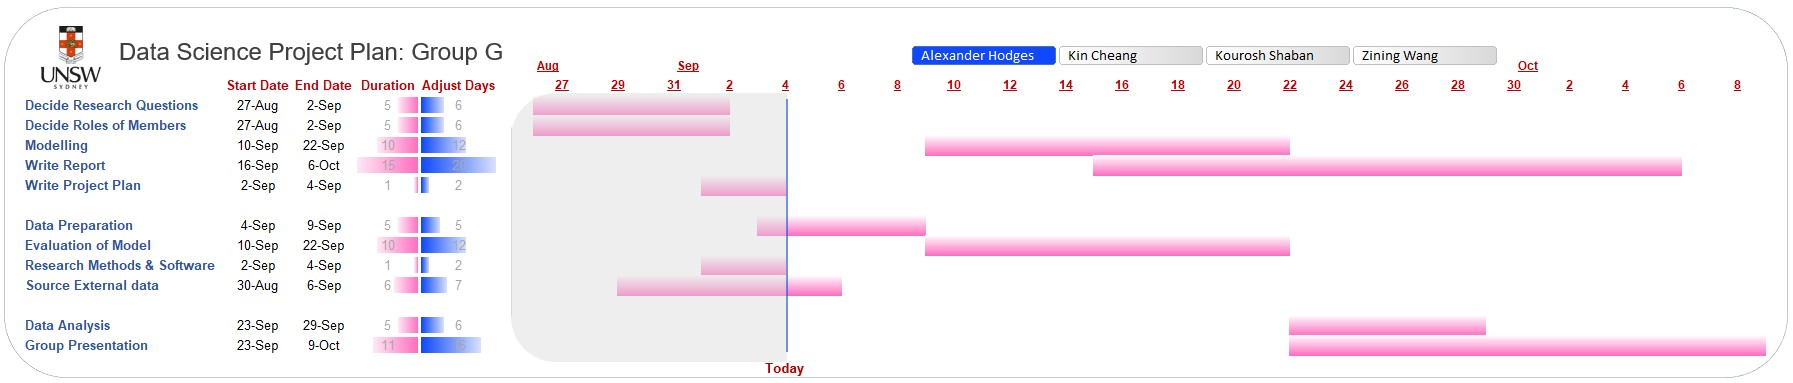
\includegraphics[scale=0.58,angle=270]{C:/Users/Josh/Desktop/GanttChart.jpg} %may need change file path, GanttChart.jpg can find in gantt_chart folder/google drive
		\caption{Project Plan and Timeline}
	\end{figure}%closing statement-body
	
%\end{document}%closing statement-body
\bigskip
%%%%%%%%%%%%%%%%%%%%%%%%%%%%%%%%%%%%%%%%%%%%%%%%%%%%%%%%%%%%%%%%%%%%%%%%%%%%%%%%%%%%%%%%%%%%%%%%%%%%%%%%%%%%%%%%%%%%%%%%%%%%%%%%%%%%%%%%%%%%%%%%%%%%%
\hypertarget{references}{%
\chapter*{References}\label{references}}
\addcontentsline{toc}{chapter}{References}

\bibliographystyle{elsarticle-num}
\bibliography{references}

\hypertarget{refs}{}

\leavevmode\vadjust pre{\hypertarget{ref-Lafaye2013}{}}%

\hangindent=2em
\hangafter=1
Abu-Rayash, A. \& Dincer, I., 2020, ‘Analysis of the electricity demand trends amidst the COVID-19 coronavirus pandemic’, Energy Research \& Social Science, vol. 68, pp.101682. \hfill\break

\hangindent=2em
\hangafter=1
\noindent Australian Energy Market Operator (AEMO) 2020, COVID-19 Demand Impact in Australia, assessed 30 August 2023, $<$https://aemo.com.au/en/newsroom/news-updates/demand-impact-australia-covid19$>$. \hfill\break

\hangindent=2em
\hangafter=1
\noindent Farrow, H. 2020, Commercial down v residential up: COVID-19’s electricity impact, Energy Networks Australia, assessed 30 August 2023, $<$https://www. energynetworks.com.au/news/energy-insider/2020-energy-insider/commercial -down-v-residential-up-covid-19s-electricity-impact/\#\_edn2$>$. \hfill\break

\hangindent=2em
\hangafter=1
\noindent Krarti, M. \& Aldubyan, M. 2021, ‘Review analysis of COVID-19 impact on electricity demand for residential buildings’, Renewable and Sustainable Energy Reviews, vol. 143, pp.110888. \hfill\break

\hangindent=2em
\hangafter=1
\noindent Santiago, I., Moreno-Munoz, A., Quintero-Jiménez, P., Garcia-Torres, F. \& Gonzalez-Redondo, M.J. 2021, ‘Electricity demand during pandemic times: The case of the COVID-19 in Spain’, Energy Policy, vol. 148, pp.111964. \hfill\break

\hangindent=2em
\hangafter=1
\noindent Snow, S., Bean, R., Glencross, M. \& Horrocks, N. 2020, ‘Drivers behind residential electricity demand fluctuations due to COVID-19 restrictions’, Energies, vol. 13, no. 21, pp.5738. \hfill\break

\hangindent=2em
\hangafter=1
\noindent Wu, J., Levi, N., Araujo, R. \& Wang, Y.G. 2023, ‘An evaluation of the impact of COVID-19 lockdowns on electricity demand’, Electric Power Systems Research, vol. 216, pp.109015. \hfill\break









\end{document}

